\documentclass{report}
\usepackage{color,soul}
\usepackage{graphicx}
\usepackage[document]{ragged2e}
\usepackage{circuitikz}
\usepackage{verbatim}
\title{P02- Working with sharelatex}
\date{2018-04-09}
\author{Pramod Banjara, 151ADB104}

\begin{document}
\maketitle
\newpage
\tableofcontents{}
\newpage
\chapter{Theoretical part}
\section{Circuit calculation} 

Calculate the voltages on the resistors shown in the diagram 1. For voltage source V1 use DC
voltage that is the last three digits of your student ID divided by 10. For example. \textcolor{red}{101REB123}
means \textcolor{red}{V1 = 12.3 (Volts)}.

\textcolor{red}{R1} is the second digit of the last 3 digits of the student ID + 1. \textcolor{red}{R2} is the last digit of the
student ID number +1. For example, if your student ID number is \textcolor{red}{101REB123} then \textcolor{red}{R1 = 3},
‘R2 = 4’.
Take a picture of the calculation. The calculation process will be required at work \textcolor{red}{P02}.
Additionally, the calculation will have to be added to the report you will complete at the end of
the semester \cite{book1}

\textcolor{red}{Circuit Diagram using circuitikz:}
\newline
\begin{circuitikz}[scale=1, every node/.style={transform shape}]
\draw
(0,2) to[R=$R1$, o-o] (4,2)
(0,2) to[C=$C$, *-*] (0,0)
(4,2) to[R=$R2$, o-o] (4,0)
(0,0) to[short, o-o] (4,0)
;
\end{circuitikz}


\section{Check modeling with gEDA}

\begin{itemize}
\item Get into the student’s work area by using ‘ssh’ on a training host with an IP address
\textcolor{red}{213.175.92.37}. For example: \textcolor{red}{ssh -X x111REB ... @ 213.175.92.37}
  \item Create a folder \underline{‘work’} and go to it. Create a folder \underline{‘P01’} and go to it
  \item Launch the program \textcolor{red}{gschem} . Create the schematics shown in the \textbf{\textit{1. }}Select the voltage
source and resistor values according to the theoretical calculation made at point \textbf{\textit{1.1.}}
Save the schematics in file called \textcolor{red}{01.sch}. Do not forget to add the ”value” parameter
to all elements. In addition, there must be a defined ”grounding point”. This is done by
assigning parameter netname = 0 to one of the connections (nets). See the lecture slides
for the usage of the program. \cite{book2}

\begin{figure}[!tb]
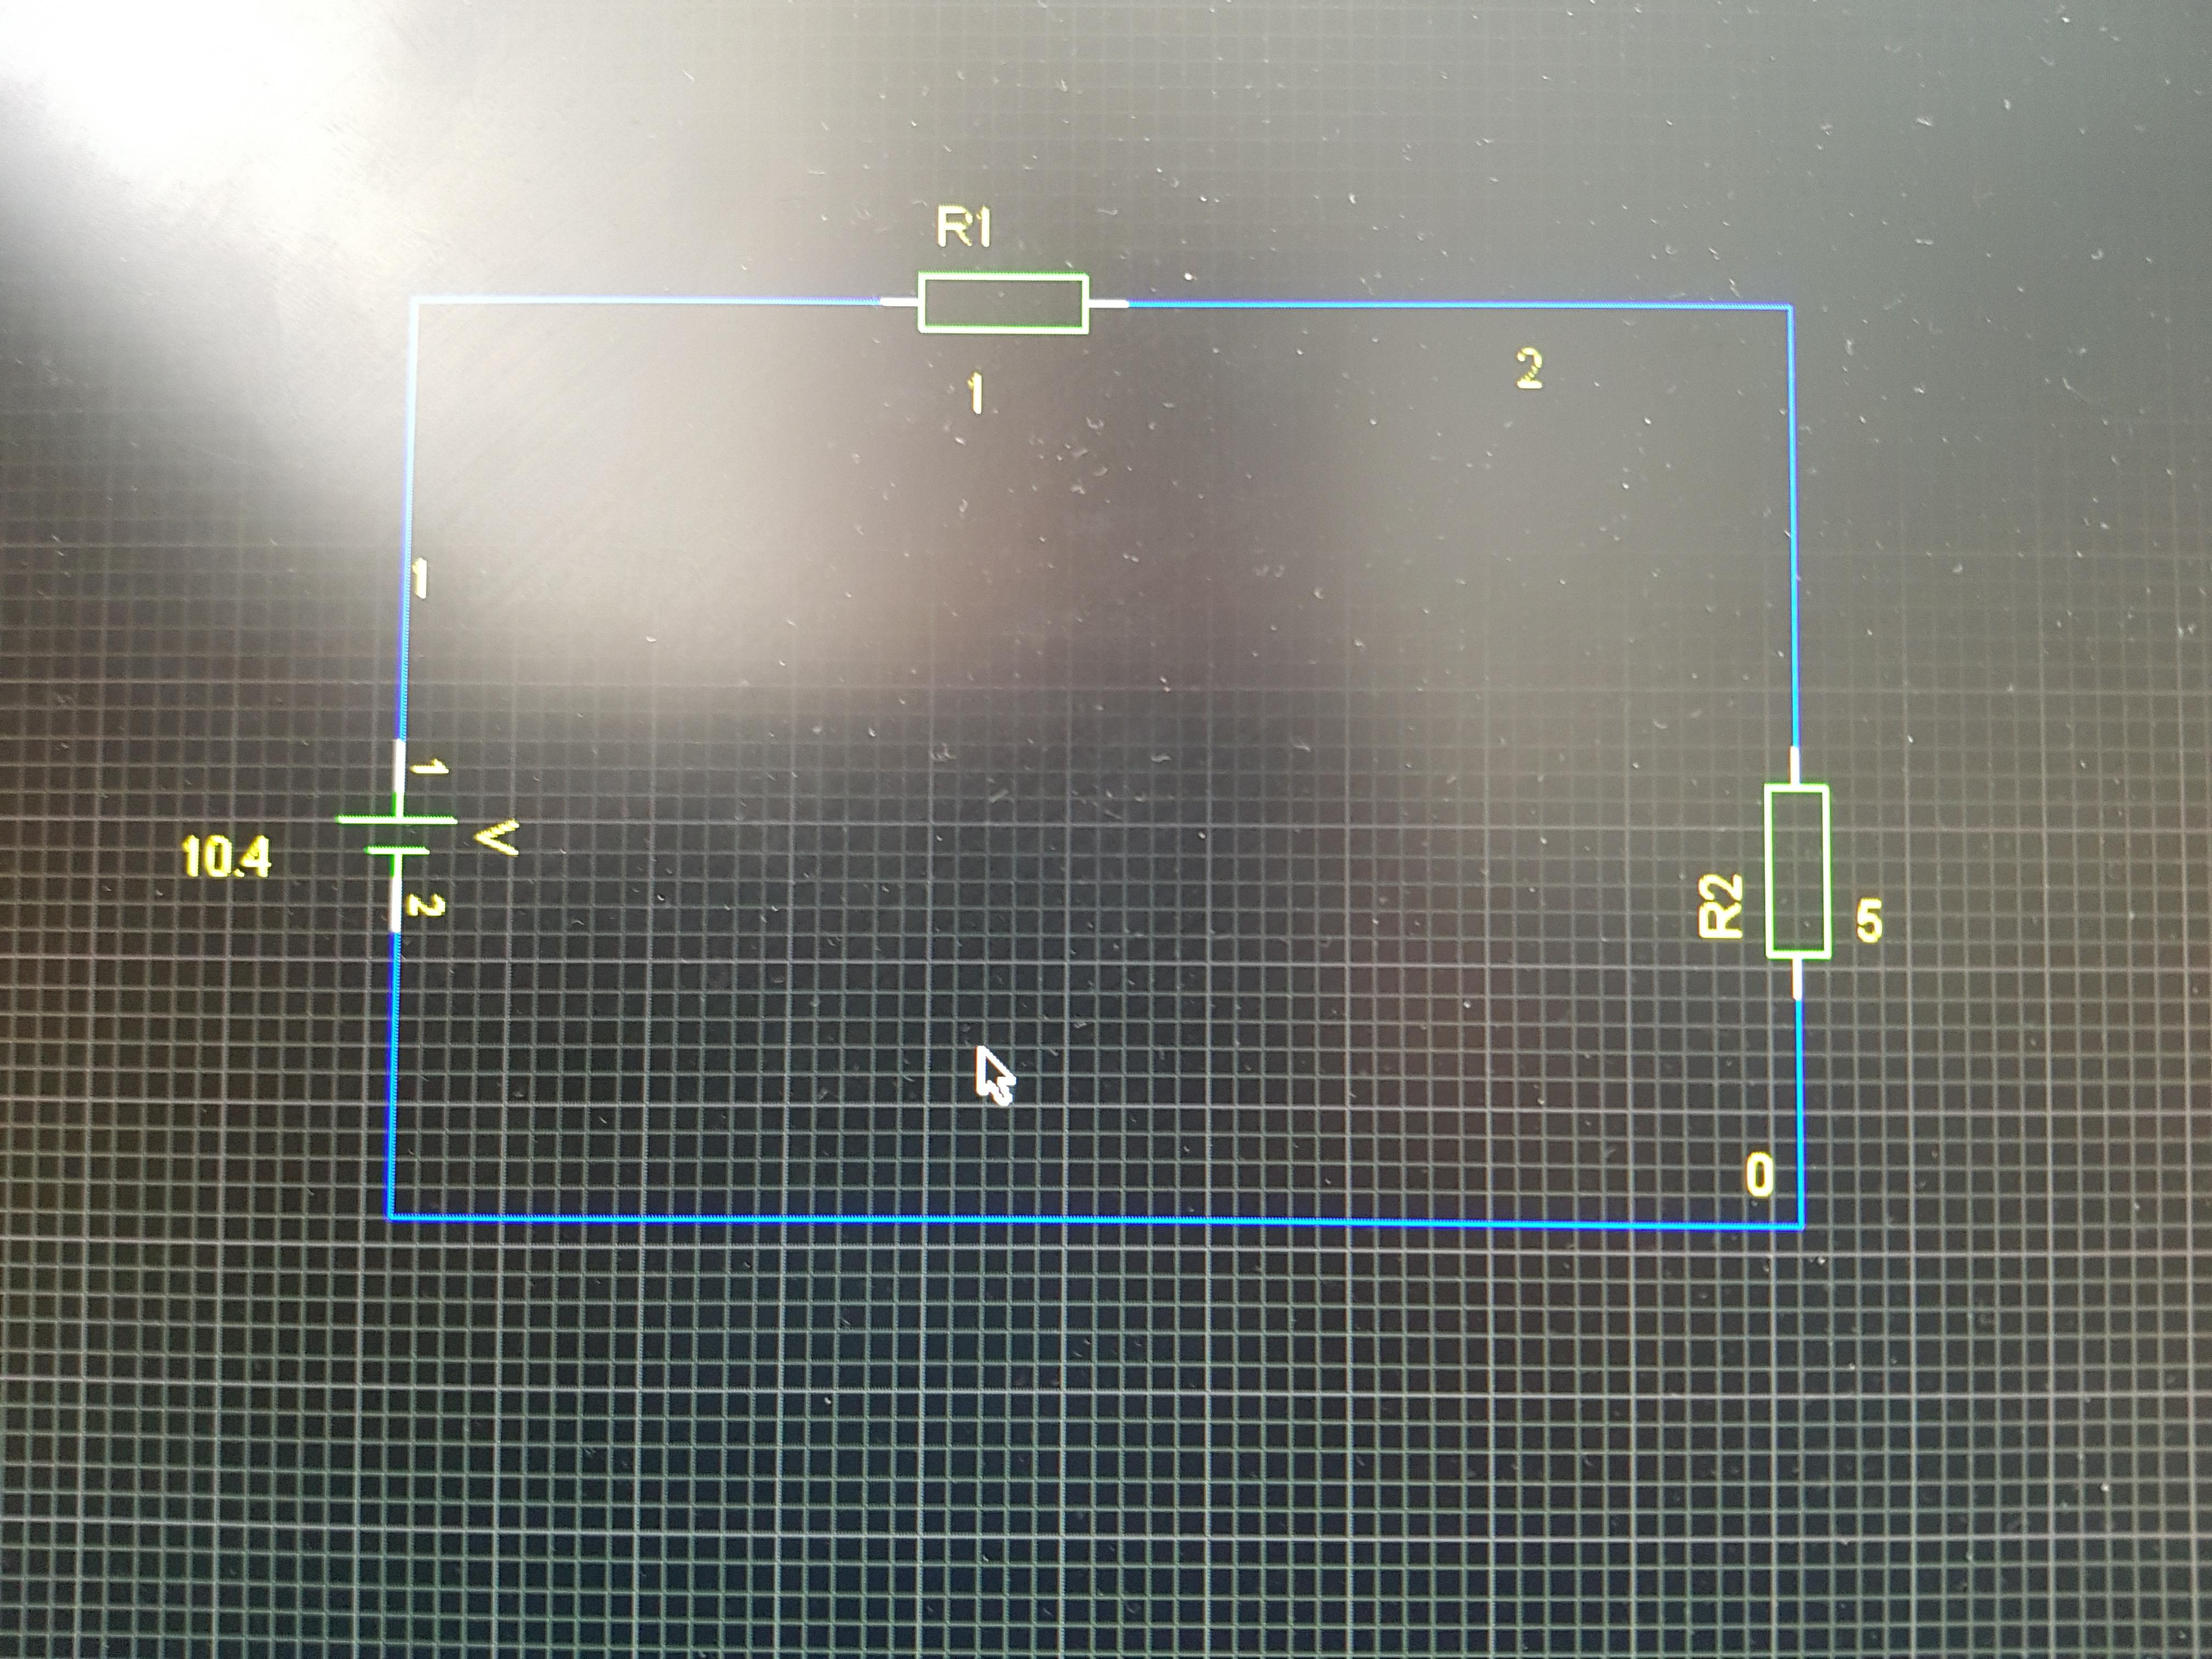
\includegraphics[width=10cm,height=10cm,keepaspectratio]{gschem-diagram.jpg}
\caption{Circuit diagram}
\end{figure}

generate the netlist file. For this purpose, run from the command line: \textcolor{red}{gnetlist -g spice 01.sch -o 01.net }.
\item Using \textcolor{red}{cat} check whether the netlist file has been generated correctly.
\item Make a simulation of the circuit ‘01.net’ using the program ‘ngspice’. For this purpose,
run \textcolor{red}{ngspice} from the command line.
\item Load the created netlist file using the command into ngspice: \textcolor{red}{source 01.net}
\item Perform a simulation of the transient process (tran) from 0 to 5 seconds in 1 second step.
\item Use plot to display the signal on the \textbf{\textit{”1”}} connection. Using \textbf{\textit{”hardcopy”}} button save
the resulting image to ‘011.png’ or make screenshot.
\item Using plot display the signal in the connection ”2”. Save the resulting image to \textbf{\textit{‘012.png’}}
or make screenshot. All this will have to be used at work ‘P02’
\end{itemize}

Bold, Italic, Underline
Some of the \textbf{greatest}
discoveries in \underline{science} 
were made by \textbf{\textit{accident}}

\section{Advanced task: Modeling with QUCS}
Start simulator QUCS. Locate the ‘Project’ menu, then select ‘Open Project’ point to
the directory ‘P01’.
\begin{itemize}
\item  Choose the tab ‘Components’ on the left. From the palette, select the two components ‘Resistor’ and the source of the component ‘DC Voltage Source’ from the ‘Sources’ menu. Put it all on the work surface as shown in the 2 image. Select the voltage source and resistor values according to the theoretical calculation at point 1.1. Make sure the visible component parameters (R1, R2, V1, etc.) are not overlapped and legible.
    \item  Use CTRL + E to turn on ”wiring” or connection mode and 0connect the components. Do not forget to add ‘Ground’ to the scheme.
\end{itemize}


\begin{figure}[!tb]
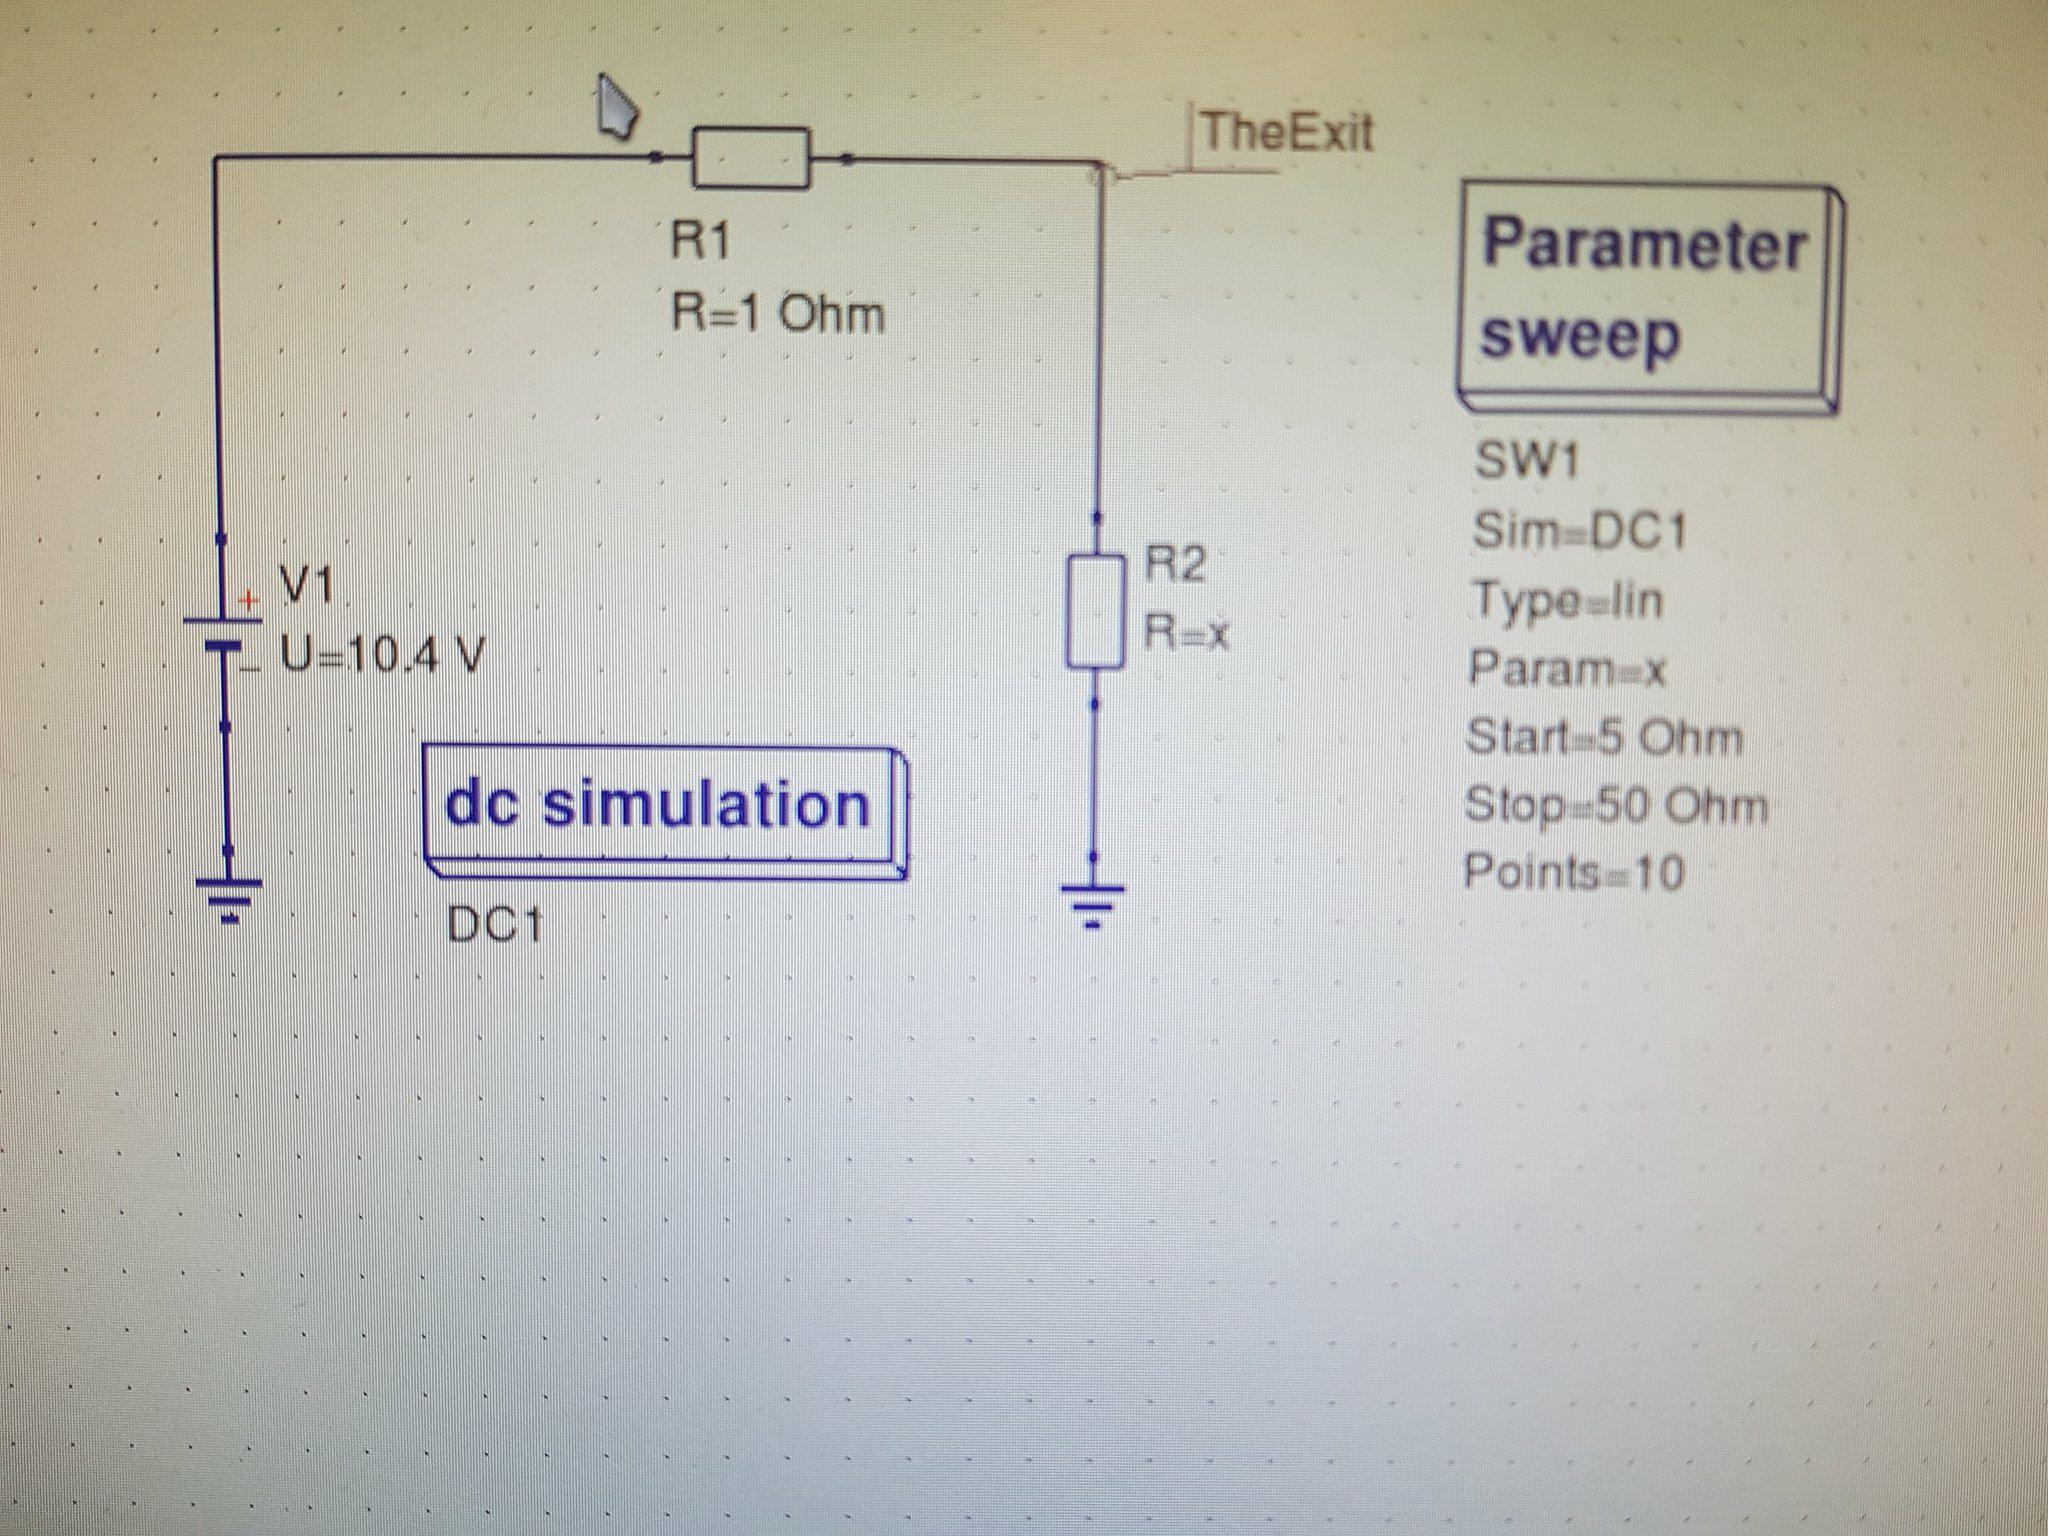
\includegraphics[width=10cm,height=10cm,keepaspectratio]{dc-sim.jpg}
\caption{The QUCS schematics environment}
\end{figure}


\begin{itemize}
\item From the menu, open the category ‘simulations’ and add the ”DC simulation” block to
your schema. Without this block, QUCS will not know what needs to be done.
\item Save the created scheme with the command sequence File-Save. Name the newly created
file as ‘02’. Qucs will add the extension (.sch) to the file itself. This will give you the
file ‘02.sch’.
\item Perform elementary DC mode simulation with the F8 key, which results in calculations
and determines the voltage on the resistor R2. The simulator variable that derives this
value is designated R2.V.
\item Add the schema to the simulation component ‘Parameter sweep’, which is selected from
the category ‘simulations’ (see Fig. 3). Evaluate the Sweep simulation attributes and
their parameters displayed on the screen.

\item Change the value of resistor R2 to the symbol x, which will serve as the argument for the
current circuit calculation. This symbol: x must also be written in the Param field of the
component ‘parameter sweep’ attribute field.
\item Change number of points to 10. Now, simulating parameter x will be changed linearly
from value 5 Ω to 50Ω at eleven points, where all the parameters of the circuit (current
and voltages) will be calculated corresponding number of times because they depend of
resistor R2 value.
\item Press F8. In the resulting parameter selection form, change them, obtain and estimate
the calculated voltage value on the resistor R2-UR2, which can be seen in the simulator
as R2.V.
\item Enhance the chain by introducing the label for wire connecting R1 to R2. Sometimes it
says: ”... the node connecting R1 to R2”. Highlight the wire and call it the exit (see Fig.
4).

 \end{itemize}

\begin{table}[!tb]
    \begin{center}
        \begin{tabular}{ |c|c|c|c| } 
            \hline
            R1  & 1 \\ 
            \hline
            R2 & 6 \\ 
            \hline
            V1 & 10.4 \\ 
            \hline
            UR1 & \\ 
            \hline
            UR2 & \\ 
            \hline
        \end{tabular}
        \caption{Table with cicuit input data}
    \end{center}
\end{table}

 
 \chapter{Practical part}
\section{Work with GEDA programs} 
check floated figure :)
\subsection{Work with gschem}
check floated figure :)

\begin{figure}[!tb]
    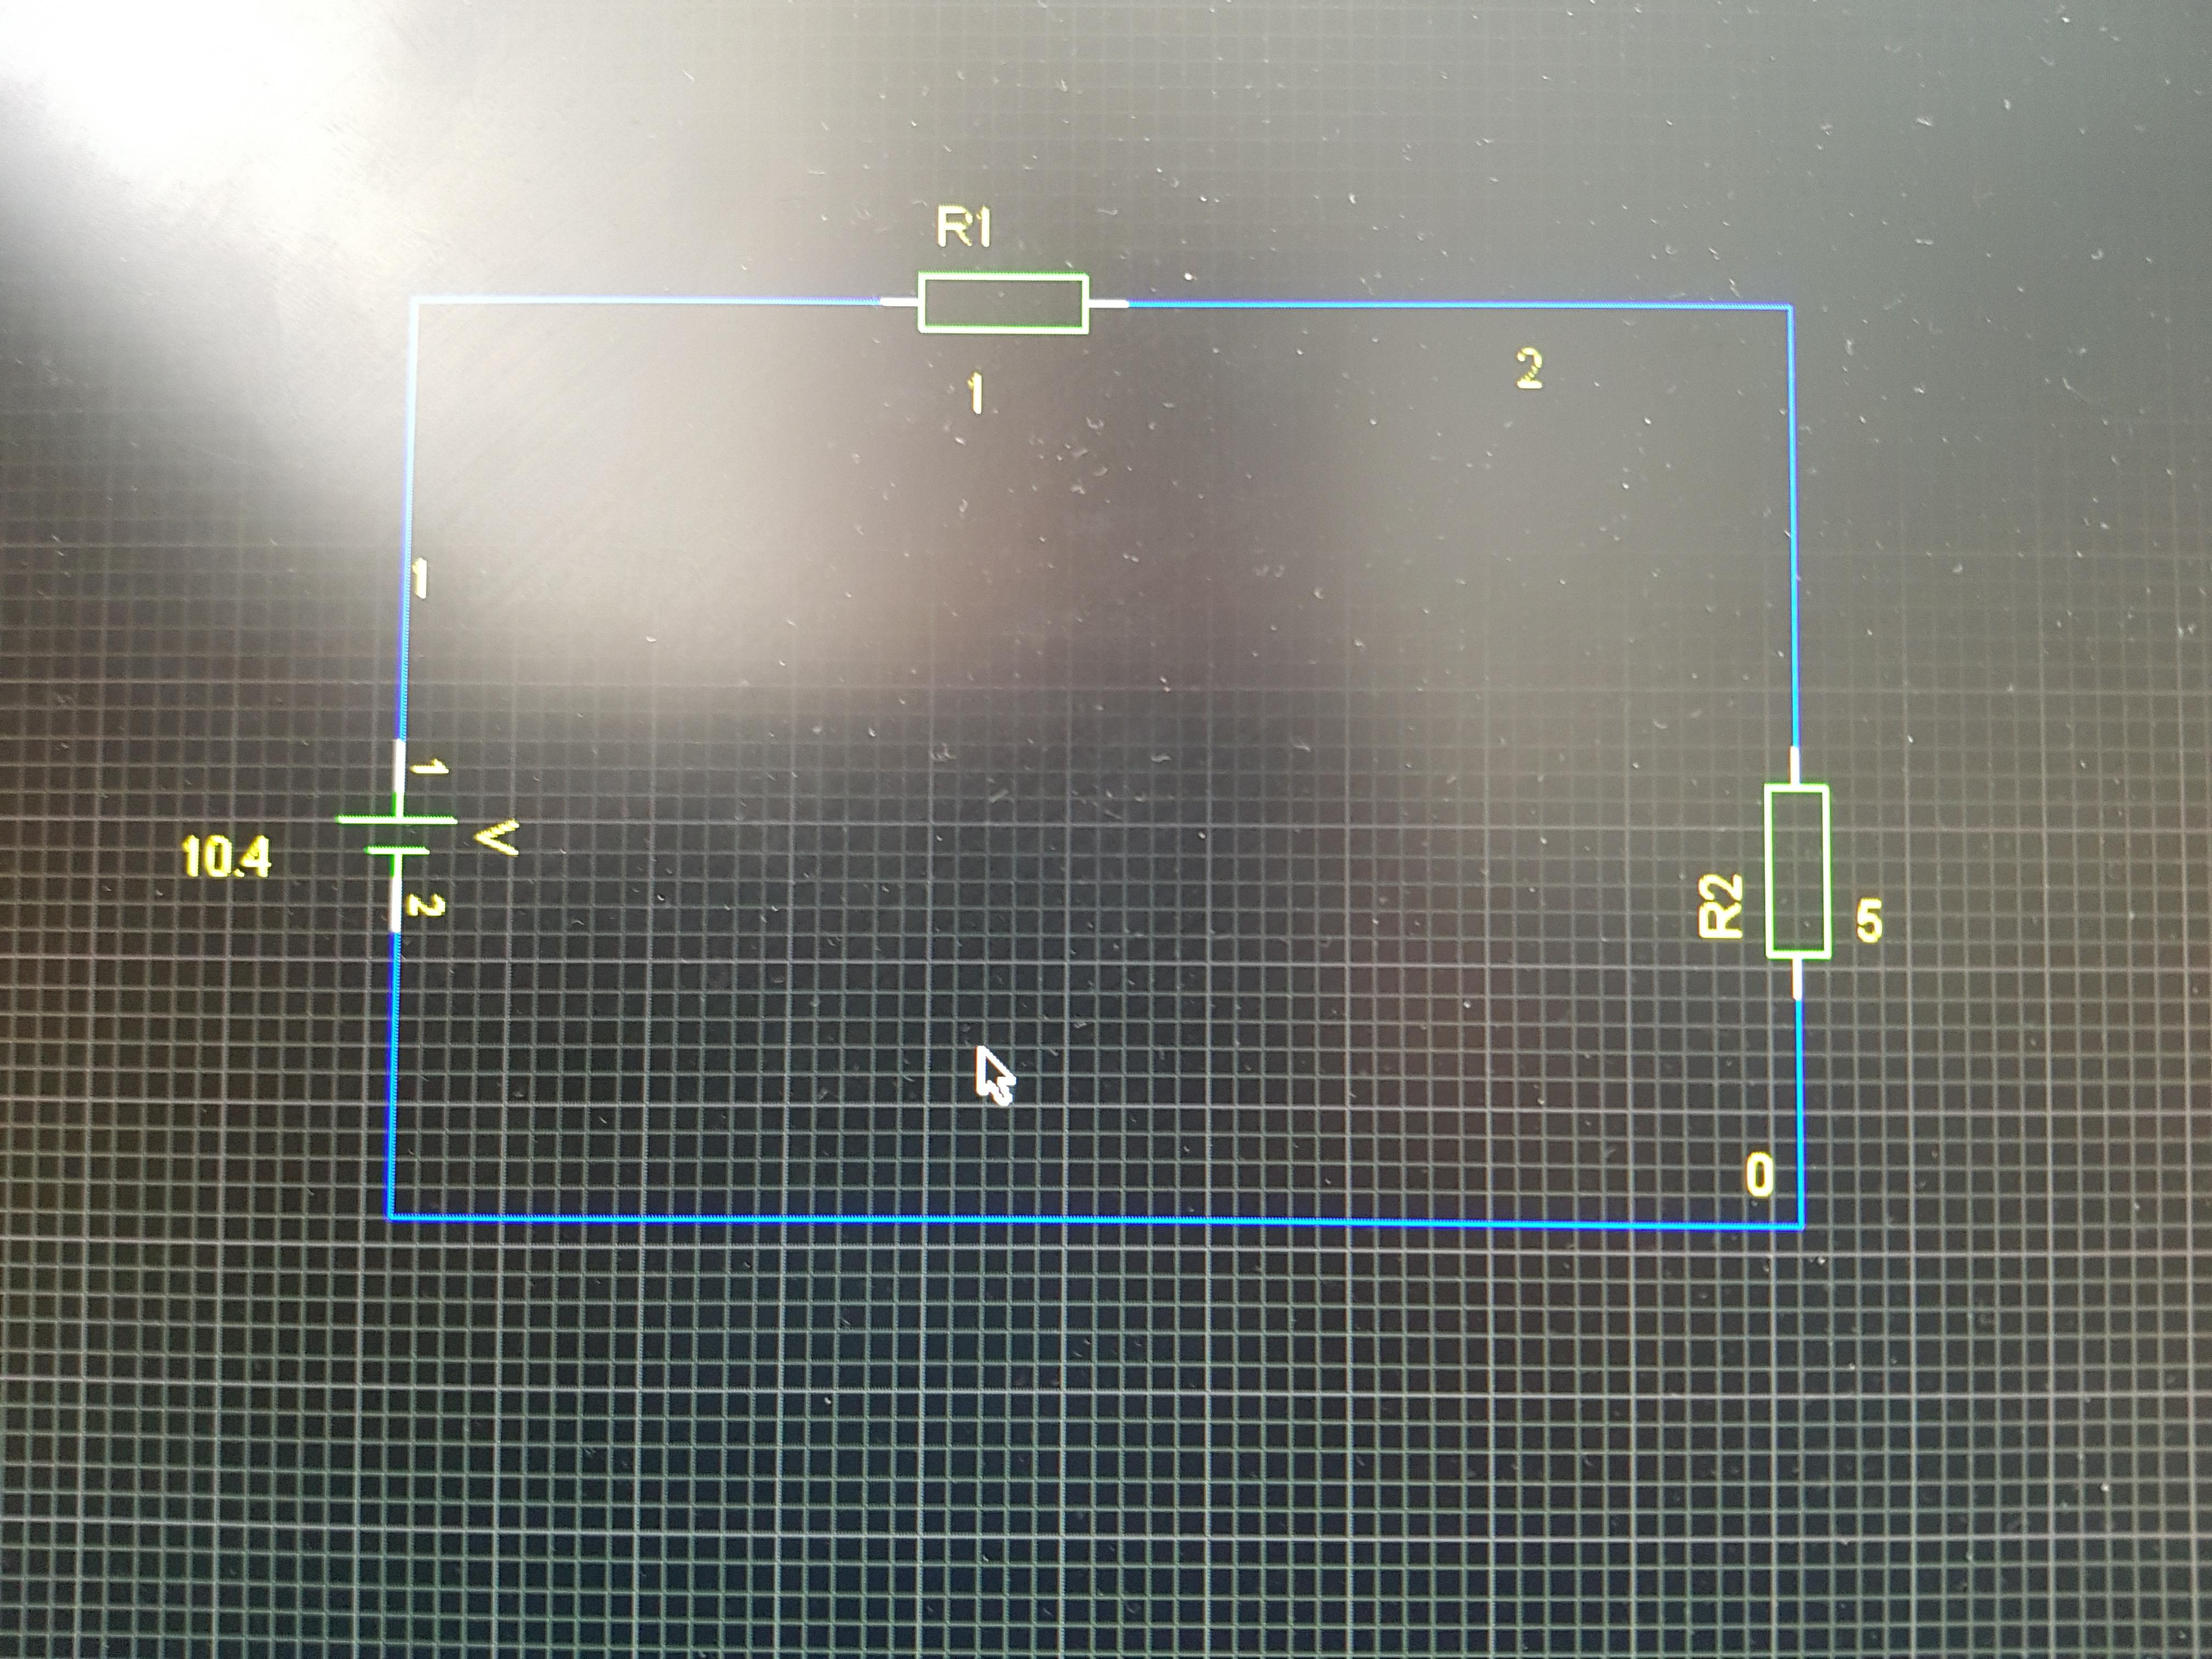
\includegraphics[width=10cm,height=10cm,keepaspectratio]{gschem-diagram.jpg}
    \caption{gschem -design of circuit}
\end{figure}

\subsection{ Work with gnetlist}

\verbatiminput{1.net}
 
 \subsection{Work with ngspice’}
 

 \begin{center}
 
 \begin{figure}[!tb]
    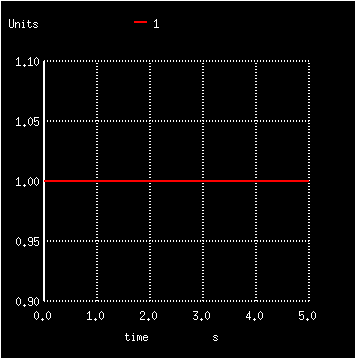
\includegraphics[width=10cm,height=10cm,keepaspectratio]{011.png}
    \caption{result of simulation 1}
\end{figure}

 \begin{figure}[!tb]
    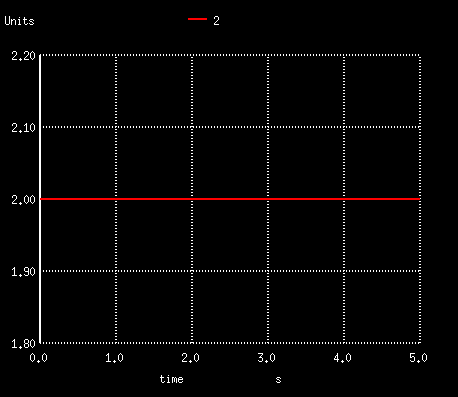
\includegraphics[width=10cm,height=10cm,keepaspectratio]{012.png}
    \caption{result of simulation 2}
\end{figure}

\end{center}





\section{Work with QUCS programs}
  \subsection{Image of the schematics}
  \begin{figure}[!tb]
    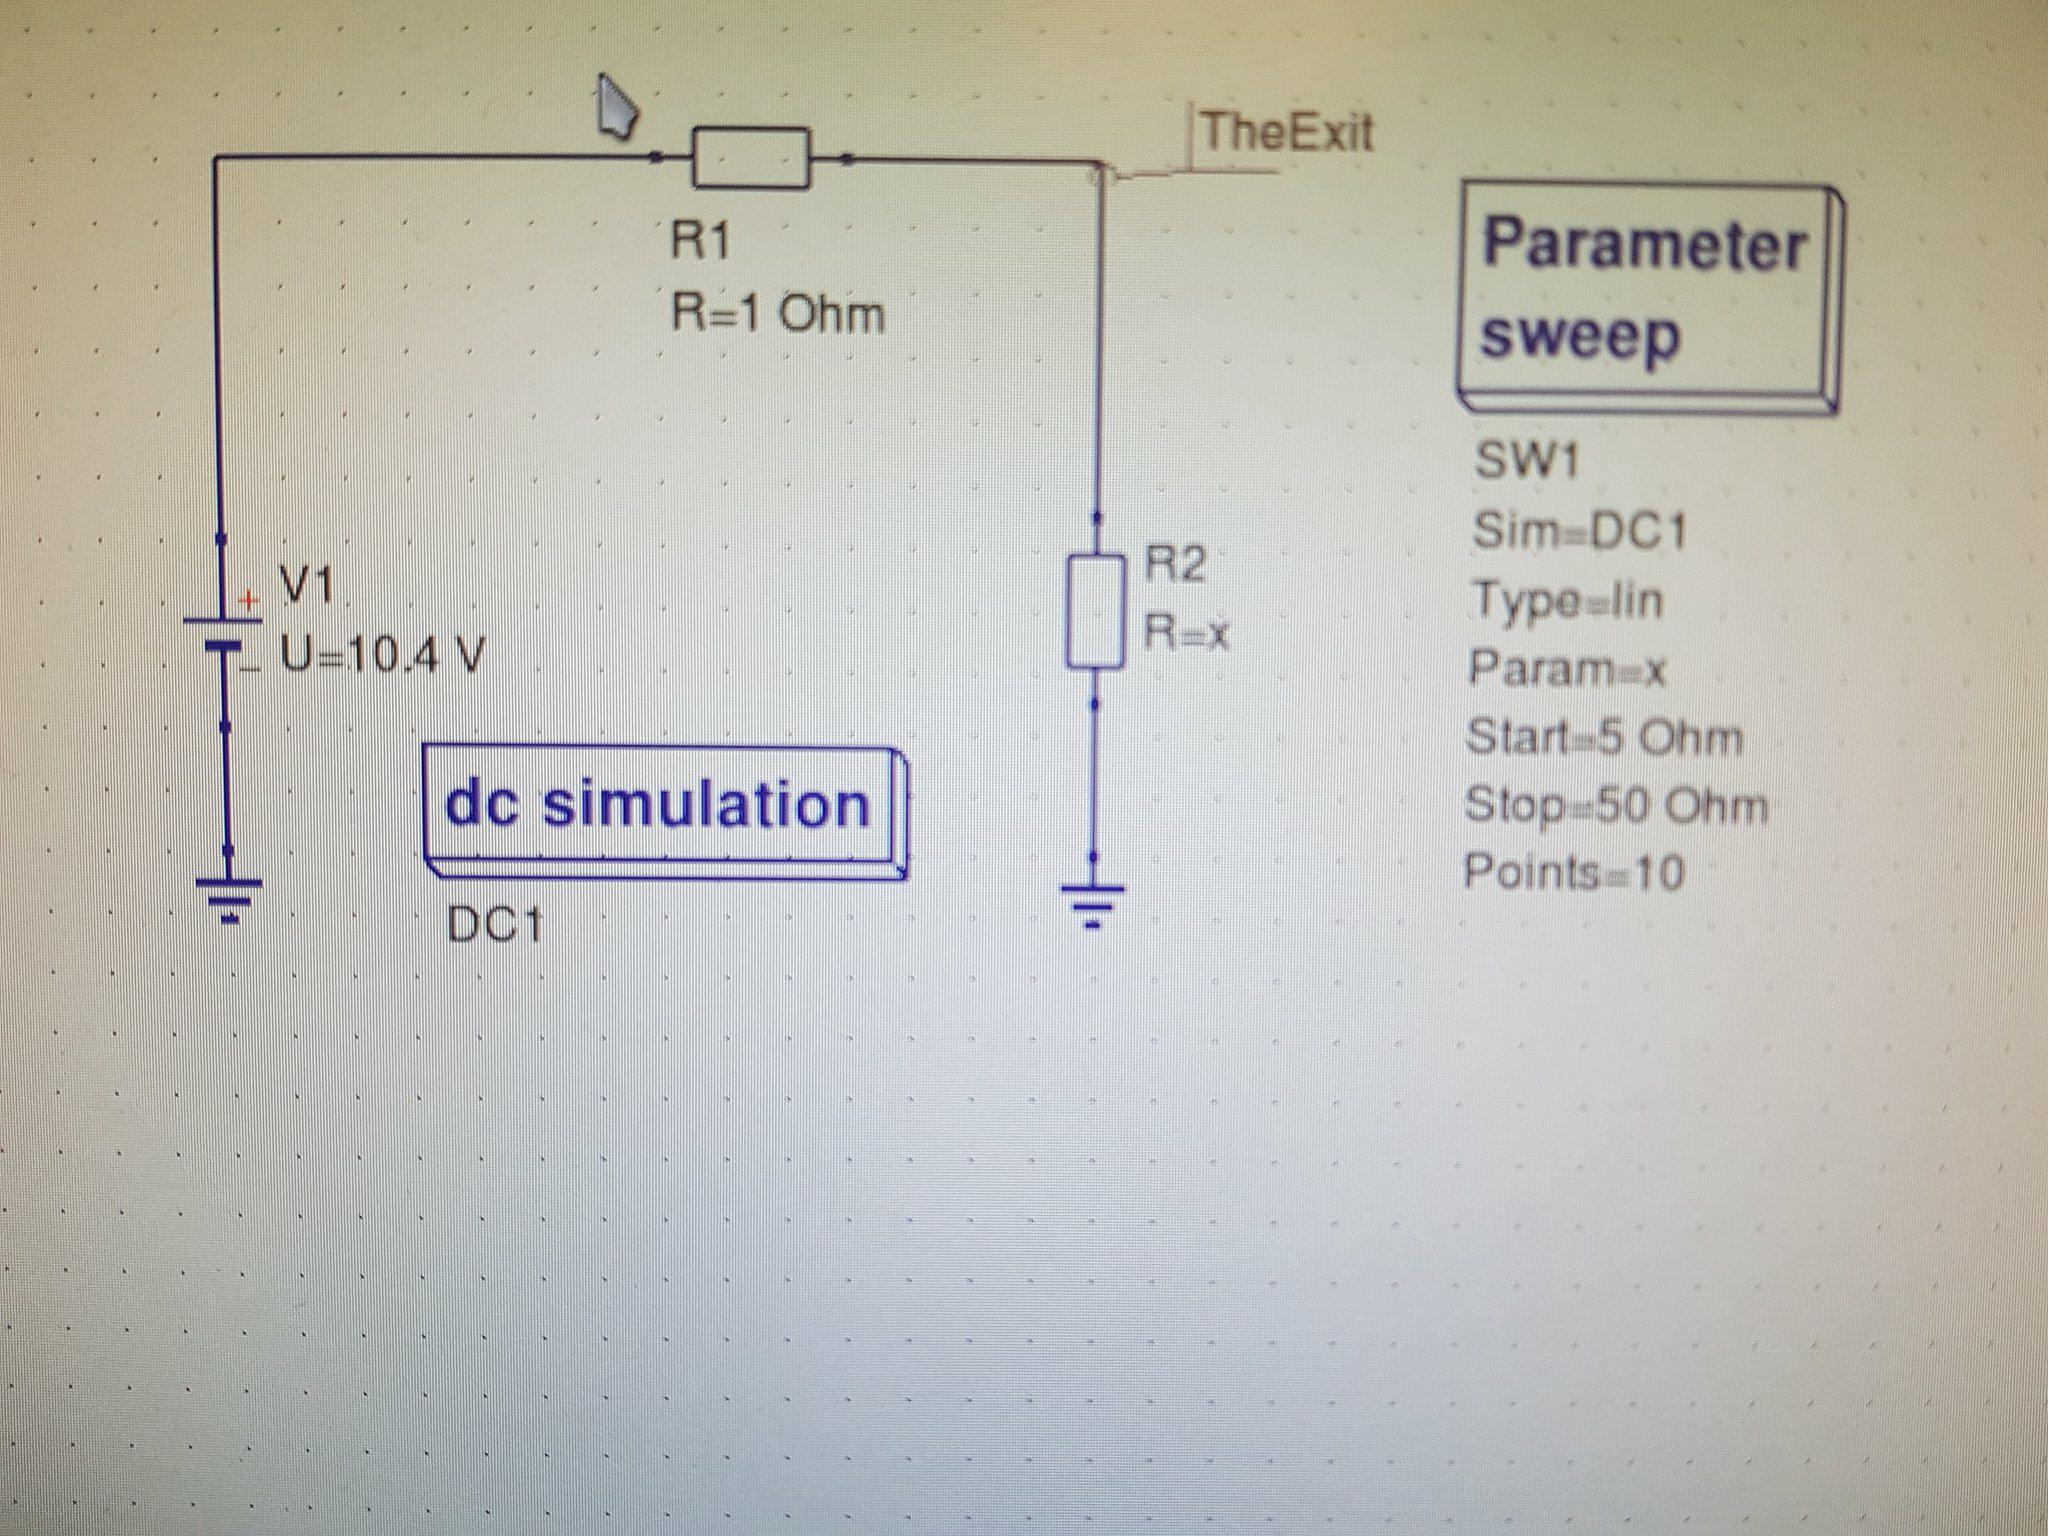
\includegraphics[width=10cm,height=10cm,keepaspectratio]{dc-sim.jpg}
    \caption{DC simulation with parameter sweep}
\end{figure}

      
  \subsection{Curve from Sweep simulation (advanced topic)}
  \begin{figure}[!tb]
    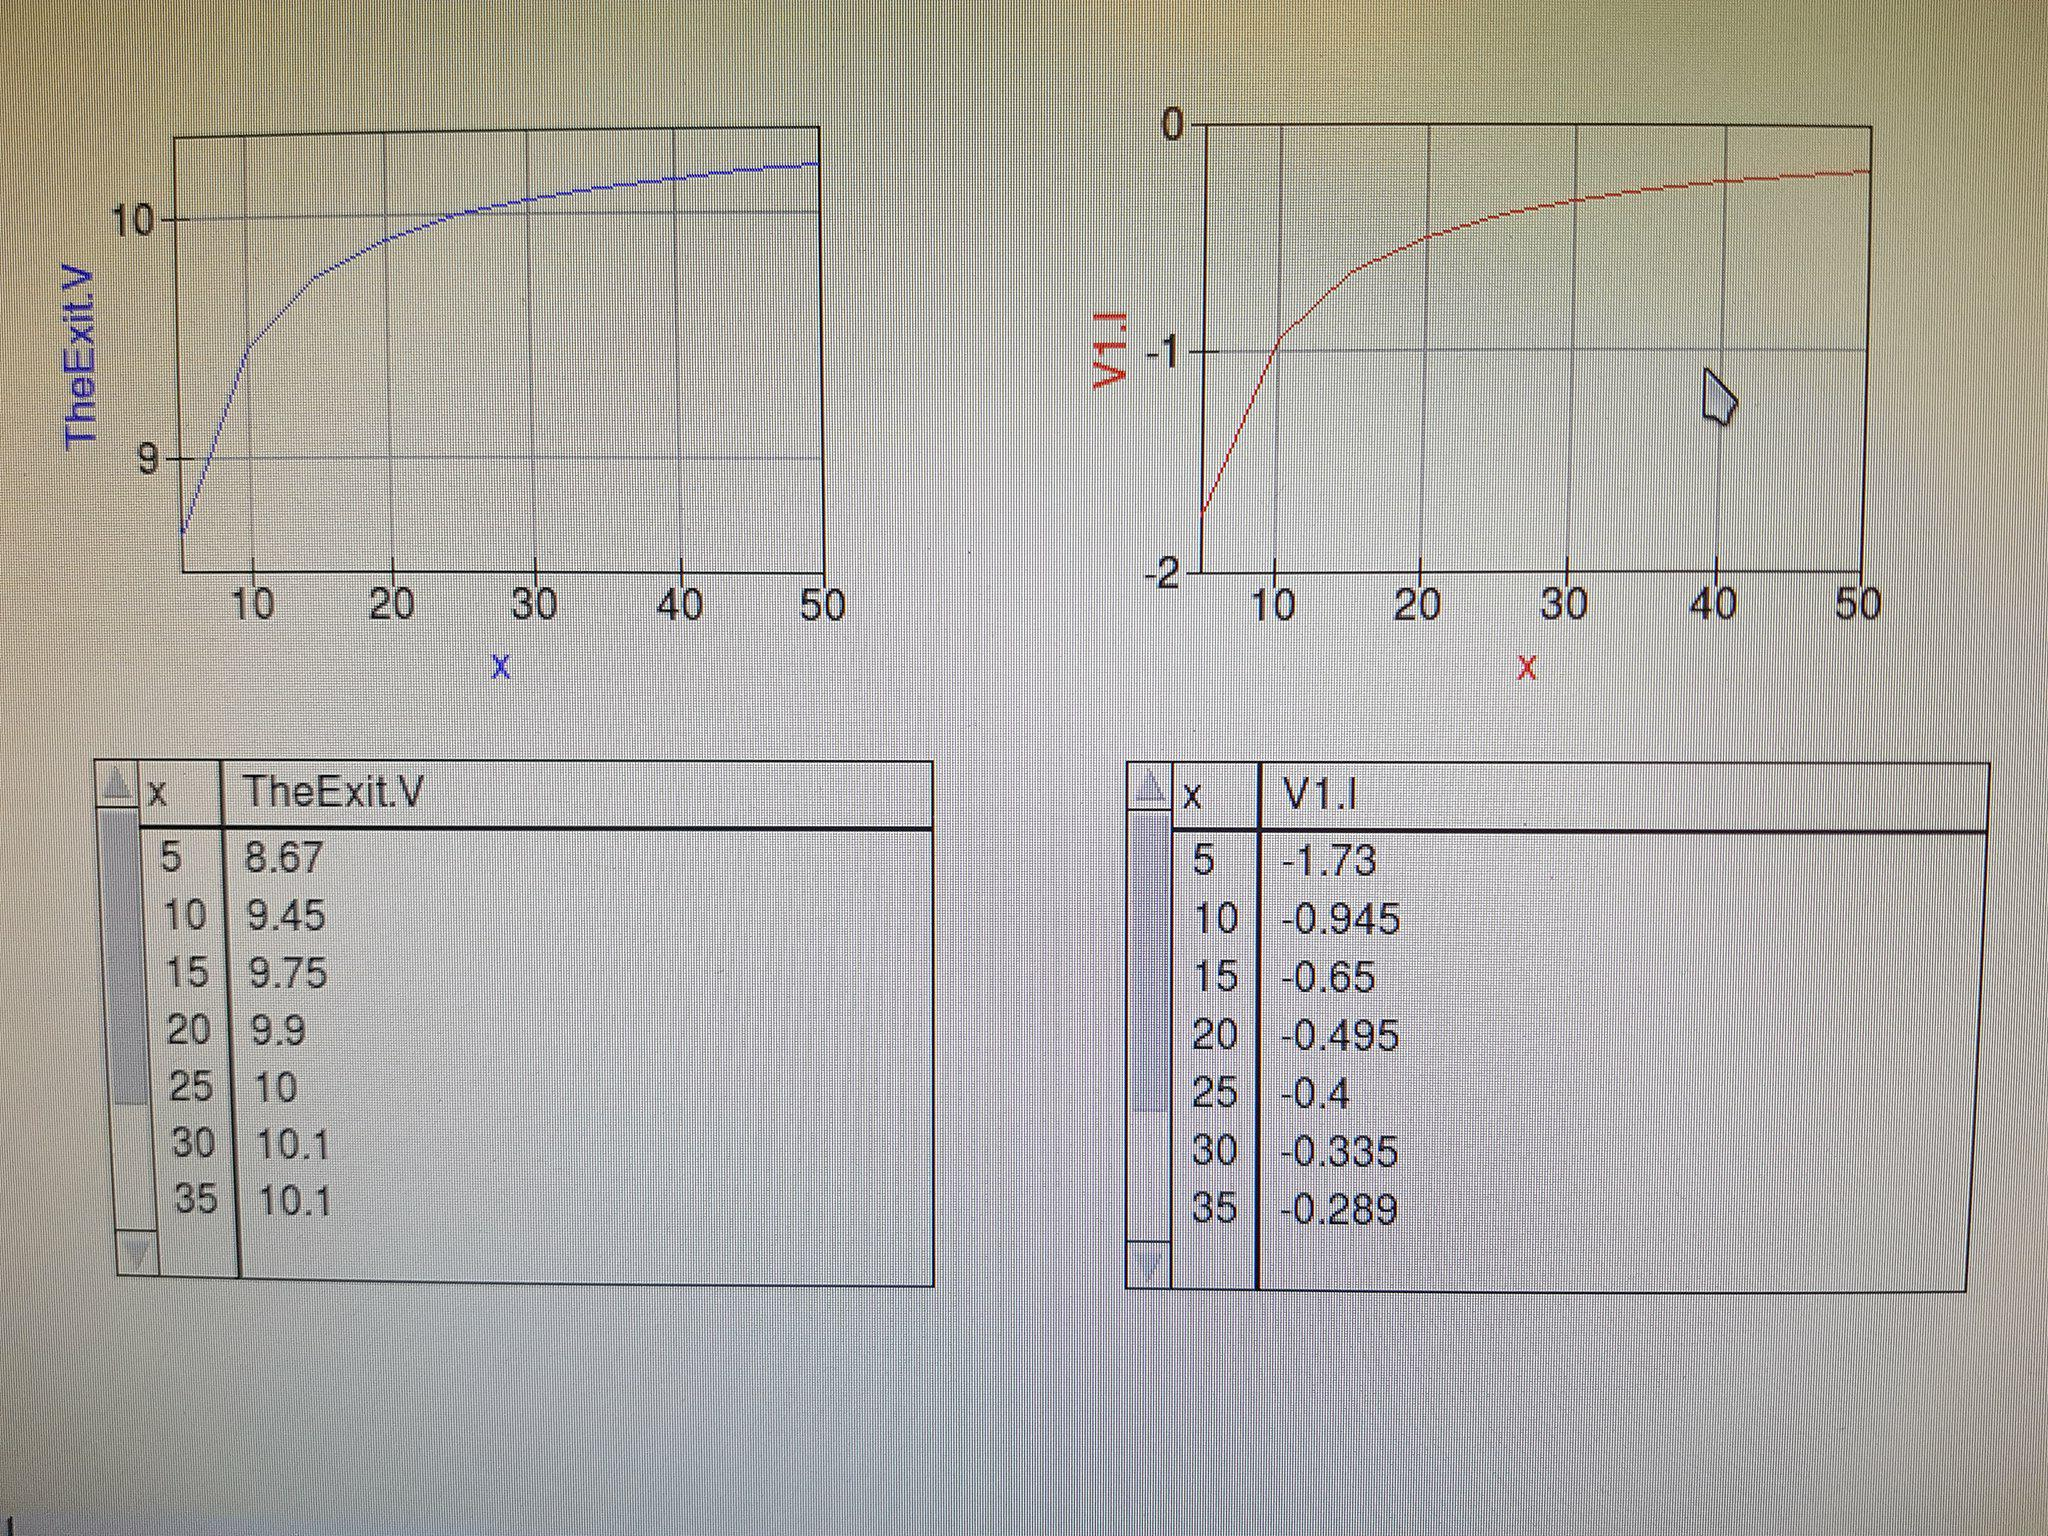
\includegraphics[width=10cm,height=10cm,keepaspectratio]{result-graph.jpg}
    \caption{Curve from sweep simulation}
\end{figure}
  \subsection{Explanations for each image and table (advanced topic)}
    write something here
    
    
\begin{thebibliography}{9}
\bibitem{book1}
M.Goossens , F.Mittelbach , and A.Samarin.
Addison -Wesley, Reading , Massachusetts , 1993.
\bibitem{book2}
La révolution antillaise: Quelle place pour l'Outre-mer dans la République? - by Luc Laventure, 2009
\end{thebibliography}

  
\end{document}